\documentclass[11pt]{article}
\usepackage[a4paper,margin=2.3cm]{geometry}
\usepackage{amsmath,amssymb,booktabs,graphicx,hyperref}
\usepackage{url}
\newcommand{\dd}{\mathrm{d}}
\newcommand{\code}[1]{\path{#1}}
\newcommand{\ket}[1]{|#1\rangle}
\sloppy
\title{Which resonance does an AGN-disk companion hit first?}
\author{Implementation note for \code{src/GW_forward/analysis/}:\\
\code{agn_cloud_resonances.py}, \code{agn_julia_pipeline.py}, \code{evolve_agn_history.jl},\\
\code{run_agn_scan.sh}, \code{agn_scan_summary.py}}
\date{}
\begin{document}
\maketitle

\section{Question}
A massive black hole (MBH) grows by episodic thin-disk accretion and hosts a scalar cloud of mass $\mu$. During an accretion episode a stellar-mass BH forms in or is captured by the disk, migrates inward on a circular, equatorial, prograde orbit, and sweeps through the gravitational-atom resonances. We record the \emph{first} transition it crosses, as a function of the boson mass, for MBHs that end up in the LISA band. The pipeline has three stages: a cheap accretion history without the boson, the full cloud evolution along that history (Julia), and a Monte Carlo over companions.

\section{Accretion histories}
Seeds form at $z=15$ (flat $\Lambda$CDM, $H_0=67.7$, $\Omega_m=0.31$) with $M_{\rm seed}$ log-uniform in $[10^2,10^5]\,M_\odot$ and $a_{\rm seed}\in[0,0.5]$. Accretion is ON in episodes of fixed length $t_{\rm ep}=10$\,Myr at a duty cycle $f\sim U[0.01,0.05]$ per MBH: $n_{\rm ep}={\rm round}(fT/t_{\rm ep})$ episodes, one per slot of length $T/n_{\rm ep}$ with a uniform start inside it ($T$ = time from the seed to today). While ON,
\begin{equation}
\frac{\dd\ln M}{\dd t}=\frac{\lambda_{\rm on}(1-\epsilon)}{\epsilon\,t_{\rm Edd}},\qquad
\frac{\dd a}{\dd\ln M}=\frac{L_{\rm isco}(a)}{E_{\rm isco}(a)}-2a ,
\end{equation}
with $\lambda_{\rm on}=0.3$, $\epsilon=0.1$, $t_{\rm Edd}=\sigma_Tc/4\pi Gm_p\simeq450$\,Myr, coherent (prograde) Bardeen spin-up capped at $a=0.998$. A history is kept only if $10^5\le M(z=0)/M_\odot\le10^7$, evaluated \emph{without} superradiance. The total growth is a factor $2$--$60$, so about $35\%$ of the draws are kept and the kept seeds are heavy ($10^{3.6}$--$10^5\,M_\odot$); light seeds need a larger $\lambda_{\rm on}$ or duty cycle. Without the boson every kept MBH reaches $a=0.998$.

\section{Cloud evolution}
\code{evolve_agn_history.jl} cuts each history into its ON and OFF segments and evolves the BH and the cloud through each with one \code{solve_system} call: $\dot M=(\dd\ln M/\dd t)\,M$ with Bardeen spin-up while ON, no accretion while OFF, and superradiance, scattering (decay constant $f_a$) and GW emission throughout, for levels up to $N_{\max}$ (\code{track_alpha} on, evolving 211 cap). The output is $M(t)$, $a(t)$ and $M_{c,nlm}(t)/M$ from the seed to today. Superradiance makes the MBH up to $\sim30\%$ lighter today than the boson-free estimate used for the band cut (\code{analyze} \code{--band_check} drops histories that leave the band).

\section{Companions}
For each evolved history, $n_{\rm inj}$ companions ($m=10\,M_\odot$) are placed at times uniform in the ON time with $z<1$. Each has a formation channel, disk capture ($r_0\in[10^3,10^6]\,r_g$) or in-situ formation ($r_0\in[10^5,10^6]\,r_g$), with equal weight and $r_0$ log-uniform. $M$ and $a$ are frozen at their values at the injection time. The orbit migrates in a steady $\alpha$-disk ($\alpha_{\rm ss}=0.01$, $h=0.01$) fed at $\lambda_{\rm on}\dot M_{\rm Edd}$: Type I ($v_r=-2C\,q\,h^{-2}\Sigma r^3\Omega/M$, $C=1.364+0.541/2$) or Type II beyond the gap-opening criterion, plus GW reaction. For these parameters the Type I time $r/|v_r|=3\pi\alpha_{\rm ss}h^4(M/\dot M)/(2Cq)$ is independent of $r$, about $4\times10^3$\,yr for $M=10^6\,M_\odot$, so companions reach $10^3\,r_g$ well within an episode. At the end of the episode the disk is removed and the orbit evolves by GWs only, stalling if it does not reach the ISCO within 1\,Gyr.

\section{Resonances}
Levels have
\begin{equation}
\frac{\omega_{nlm}}{\mu}-1=-\frac{\alpha^2}{2n^2}-\frac{\alpha^4}{8n^4}+\left(\frac{2}{n}-\frac{6}{2l+1}\right)\frac{\alpha^4}{n^3}+\frac{16\,a\,m\,\alpha^5}{2l(2l+1)(2l+2)\,n^3},
\end{equation}
and a transition $i\to f$ is resonant when the orbital frequency equals
\begin{equation}
\Omega_{\rm res}=\frac{\omega_f-\omega_i}{m_f-m_i},\qquad r_{\rm res}=(GM/\Omega_{\rm res}^2)^{1/3},
\end{equation}
with $\Omega_{\rm res}>0$ for orbits co-rotating with the cloud (all companions here). A transition is kept if a tidal multipole $l_*\in L$ couples it: $|l_i-l_f|\le l_*\le l_i+l_f$, $l_i+l_f+l_*$ even, $|\Delta m|\le l_*$, and $l_*+\Delta m$ even for an equatorial orbit. Default $L=\{2,3\}$ (\code{--l_stars}~2 for quadrupole only). Kinds: \emph{hyperfine} (same $n,l$), \emph{fine} (same $n$, different $l$), \emph{Bohr} (different $n$, final $n\le l_i+\max L+2$, which includes the lowest-$n$, i.e.\ outermost, line of every $\Delta m$). Only levels with $M_c/M\ge10^{-6}$ at the crossing count. The first crossed line is recorded (lines degenerate with it are grouped); otherwise the outcome is \emph{no cloud}, \emph{no line ahead} or \emph{stalled}. The bookkeeping is kinematic: no couplings or Landau--Zener probabilities, and no back-reaction on the cloud or the orbit.

For the 211 cloud with the spin near threshold, $\tilde a\simeq a_c(\alpha)=4\alpha/(1+4\alpha^2)$, the scalings are
\begin{align}
r_{\rm hf}^{211\to21\bar1}&=\left(\frac{12}{\tilde a\,\alpha^6}\right)^{2/3}r_g\propto\alpha^{-14/3},\qquad
r_{\rm fine}\propto\alpha^{-10/3},\\
r_{\rm Bohr}&\simeq\frac{7.7}{\alpha^2}\,r_g\ (211\to433,\ l_*=2),\qquad \frac{9.3}{\alpha^2}\,r_g\ (211\to544,\ l_*=3),
\end{align}
so the Bohr lines sit at about twice the cloud radius ($4/\alpha^2\,r_g$). The hyperfine line lies at $10^6\,r_g$ for $\alpha\simeq0.06$, $10^5\,r_g$ for $\alpha\simeq0.10$ and $10^3\,r_g$ for $\alpha\simeq0.28$. Below $\alpha\approx0.06$ every companion therefore forms inside it, and the first line it meets is Bohr; above $\alpha\approx0.1$ in-situ companions always cross the hyperfine line first.

\section{\texorpdfstring{Demo: $\mu=3\times10^{-17}$\,eV}{Demo: mu = 3e-17 eV}}
Twelve histories ($\alpha=0.225$ at $10^6\,M_\odot$; local $\alpha$ at injection 0.004--0.20), $N_{\max}=3$, 20 companions each (\code{src/GW_forward/analysis/test_run_forward/}):

\begin{center}
\begin{tabular}{lcc}
\toprule
first outcome & $L=\{2,3\}$ & $L=\{2\}$ \\
\midrule
no cloud & 51.2\% & 51.2\% \\
Bohr & 35.0\% & 34.2\% \\
hyperfine & 10.0\% & 10.0\% \\
fine & 2.5\% & 2.5\% \\
no line ahead & 1.2\% & 2.1\% \\
\bottomrule
\end{tabular}
\end{center}

\noindent The Bohr line is mostly $\ket{211}\to\ket{544}$ for $L=\{2,3\}$ and $\ket{211}\to\ket{433}$ for $L=\{2\}$; the hyperfine lines are $\ket{211}\to\ket{21\bar1}$ and $\ket{322}\to\ket{320}$ in equal numbers. \emph{No cloud} comes from MBHs at $\alpha\le0.04$ (median 0.024), where the cloud has not grown. Bohr-first companions orbit MBHs at median $\alpha=0.05$ (most within 0.04--0.07), as expected from the hyperfine radius above; hyperfine- and fine-first ones sit at $\alpha=0.07$--$0.20$ (median 0.12). Which Bohr line comes first depends on $L$, the Bohr share does not.

\begin{figure}[h]
\centering
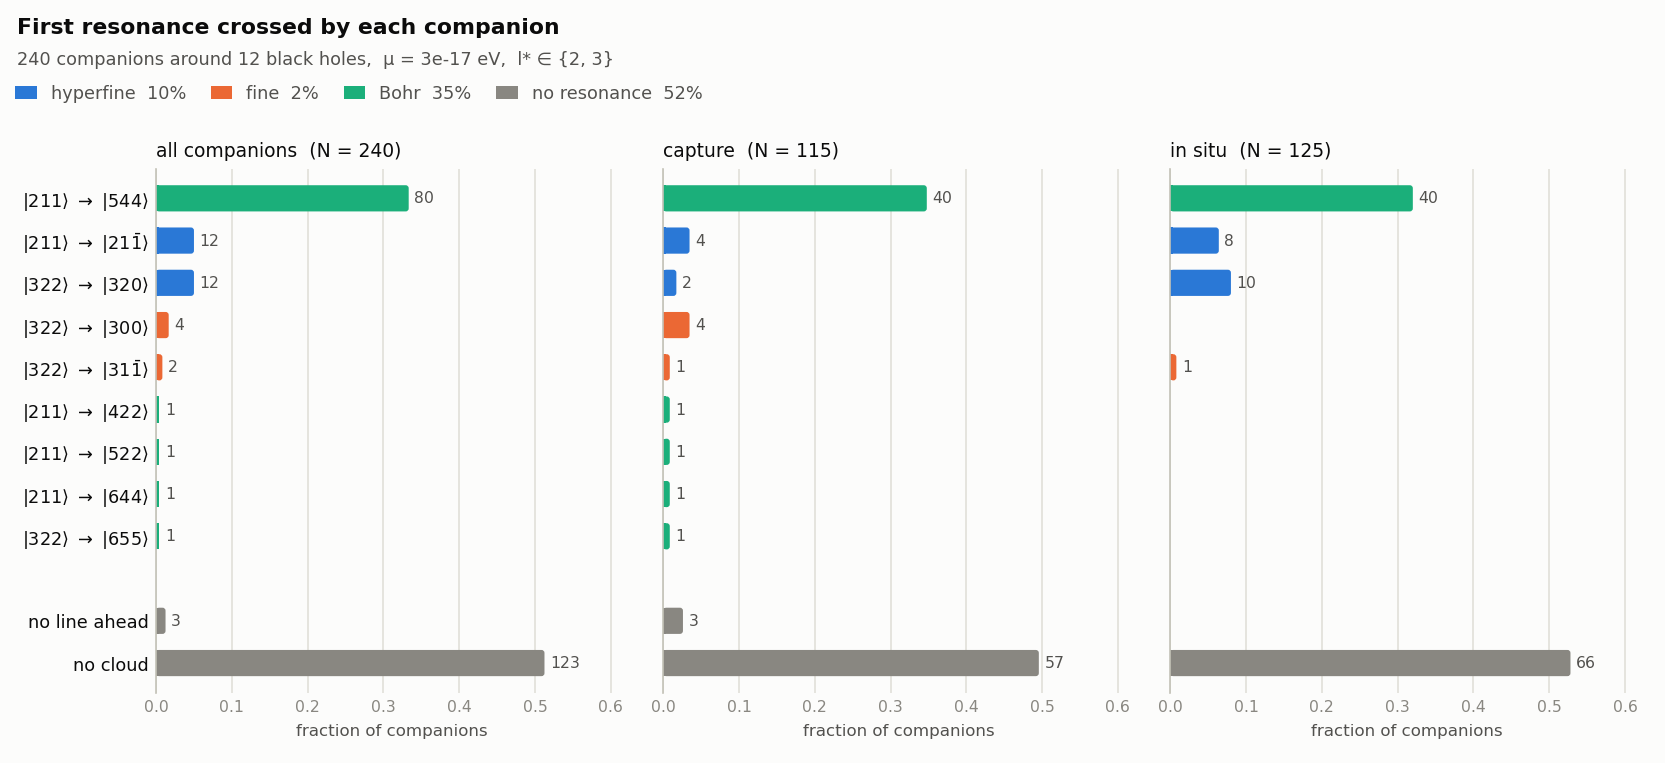
\includegraphics[width=\textwidth]{first_resonance_demo.png}
\caption{First transition crossed per companion in the demo run, for all companions and per formation channel.}
\end{figure}

\section{Running a scan}
\begin{verbatim}
cd src/GW_forward/analysis
./run_agn_scan.sh -j <cores> -N 100 -n 20 -m 4 [-q] 0.05 0.1 0.2 0.3 0.5
\end{verbatim}
Each argument is $\alpha$ at $M_{\rm ref}=10^6\,M_\odot$ (\code{-r}), one run directory per value under \code{scan_runs/}, with the same histories for every $\alpha$ (same seed). All histories share one pool of single-threaded Julia jobs; re-running the same command resumes. The output is a per-transition histogram for every $\alpha$ (\code{alpha*/first_resonance_hist.png}), plus \code{scan_summary.png} and \code{scan_kinds.csv}, \code{scan_transitions.csv}. The summary plots the outcome fractions against $\alpha$ and a transition$\times\alpha$ map; \code{-q} repeats the analysis with quadrupole tides only. Cost in the demo: 15--40\,min per history on one core at $N_{\max}=3$, several times more at $N_{\max}=4$--5.

\paragraph{What to look for.} The hand-over from Bohr-first to fine/hyperfine-first as $\alpha$ grows, and its dependence on the channel (the $r_0$ ranges); the switch from 211 to 322 lines; the \emph{no cloud} fraction at small $\alpha$; and the sensitivity to $L$, $\lambda_{\rm on}$ and the duty cycle.

\paragraph{Open issues.} (i) A coupling or Landau--Zener criterion to keep only lines that move population; (ii) companion back-reaction (floating, ionization); (iii) retrograde or misaligned companions (chaotic accretion is not supported by the Julia side); (iv) migration resuming in later episodes.

\end{document}
